\chapter{Mô tả phương pháp bằng dữ liệu mô phỏng}
Trong phần này, khóa luận minh họa dáng điệu tiệm cận của các ước lượng của các tham số và hàm hồi quy trên dữ liệu mô phỏng.

\section{Dữ liệu mô phỏng} 
Ta xét dữ liệu tuân theo mô hình \tref{1.1}
$$
Y_{i, j}=a_{j} f\left(X_{i}-\theta_{j}\right)+v_{j}+\varepsilon_{i, j}
$$
trong đó $1 \leq j \leq p$ và $1 \leq i \leq n$ với $p=5$ và $n=2000$. Ta chọn các tham số chiều cao $v=(0,1 / 3,-1,2,-9 / 10)^{T}$, các tham số chuyển $\theta=(0,1 / 5,-1 / 20,-1 / 7,1 / 6)^{T}$ và các tham số co giãn $a=(1,-4,3,-5 / 2,2)^{T}$. Thêm vào đó, nhiễu $\left(\varepsilon_{i, j}\right)$ là một dãy biến ngẫu nhiên độc lập cùng phân phối $\mathcal{N}(0,1)$. Các biến ngẫu nhiên $\left(X_{i}\right)$ được mô phỏng  theo phân phối đều trên $[-1 / 2 ; 1 / 2]$ và hàm hồi quy có $f_{1}=1 / 2$, cho bởi, với mọi $x \in[-1 / 2 ; 1 / 2]$
$$
f(x)=\sum_{k=1}^{5} \cos (2 k \pi x).
$$
Dữ liệu mô phỏng được minh họa trong hình \ref{simulatedata}. Các kết quả của các ước lượng cho các vector $v, \theta$ và $a$ bởi $\widehat{v}_{n}, \widehat{\theta}_{n}$ và $\widehat{a}_{n}$ được minh họa trong \ref{convergence}. Các giá trị đúng được xác định hướng của trục hoành và ước lượng của chúng được xác định dựa theo trục tung. Ta có thể thấy được rằng các giá trị đúng và ước lượng của chúng rất gần nhau, chứng tỏ rằng quy trình ước lượng tham số hoạt động tốt trên tập dữ liệu mô phỏng.

\begin{figure}[ht]
  \centering
  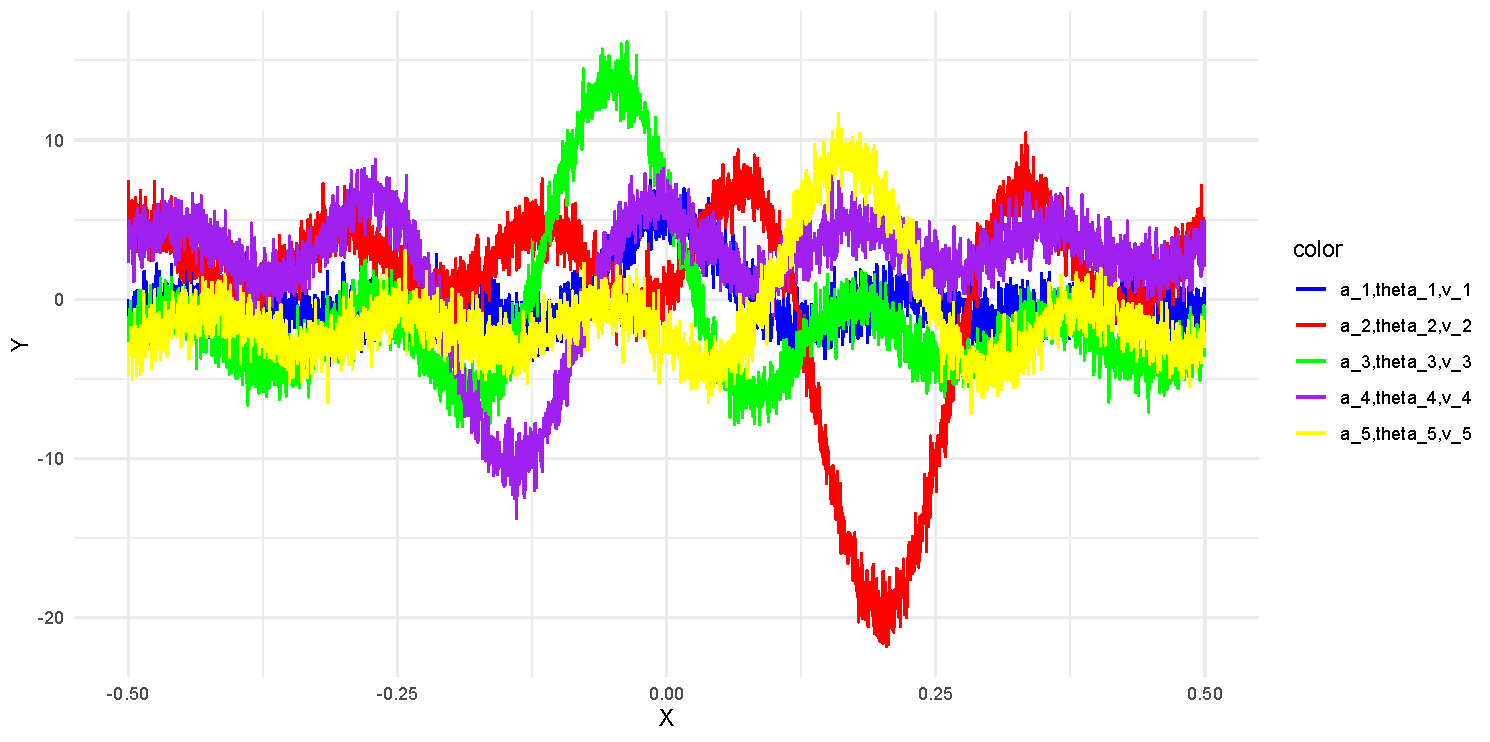
\includegraphics[width=0.65\textwidth]{Mau SP NCKH/image/Stimulated_data_vector_image.pdf}
  \caption{Dữ liệu mô phỏng}
  \label{simulatedata}
\end{figure}

\begin{figure}[ht]
  \centering
  \begin{subfigure}[b]{0.45\textwidth}
    \centering
    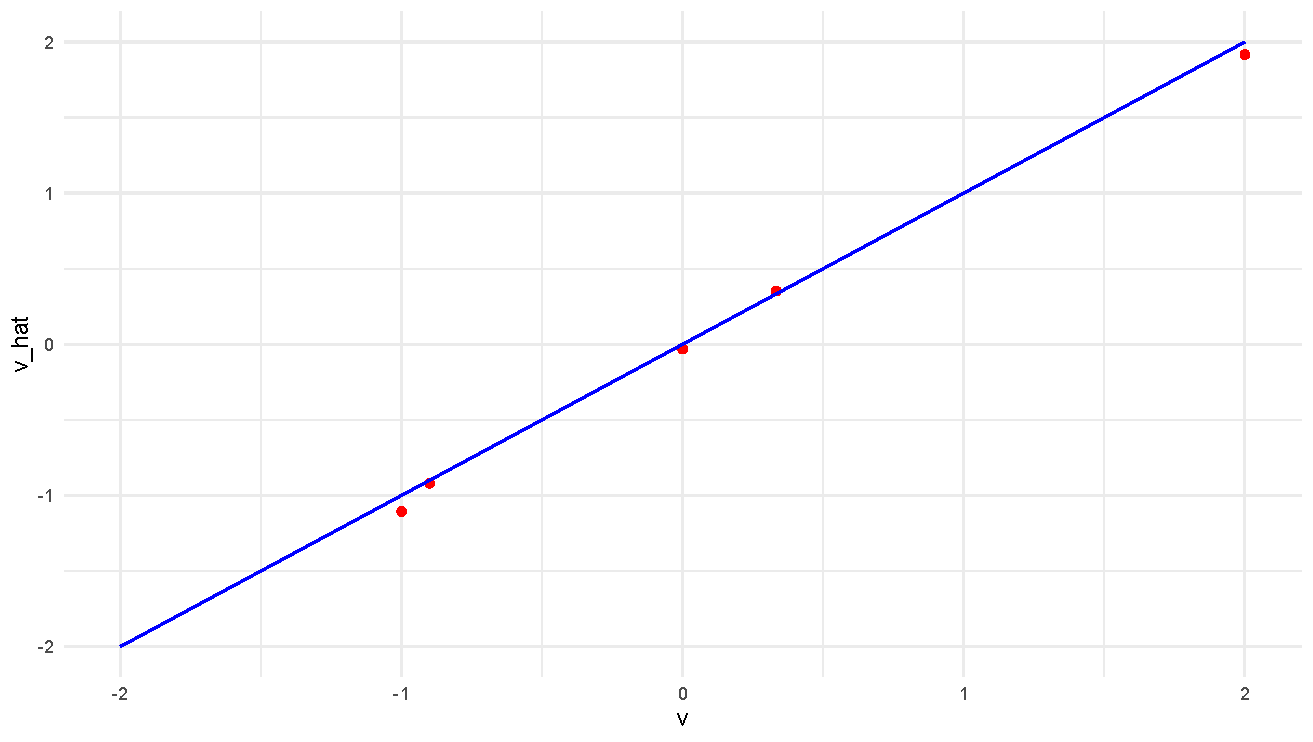
\includegraphics[width=0.8\textwidth]{Mau SP NCKH/image/Approx_v_with_v_nhat2000.pdf}
    \caption{Tham số chiều cao $v$}
    \label{fig:image3}
  \end{subfigure}
  \hfill % optional; add some horizontal spacing
  \begin{subfigure}[b]{0.45\textwidth}
    \centering
    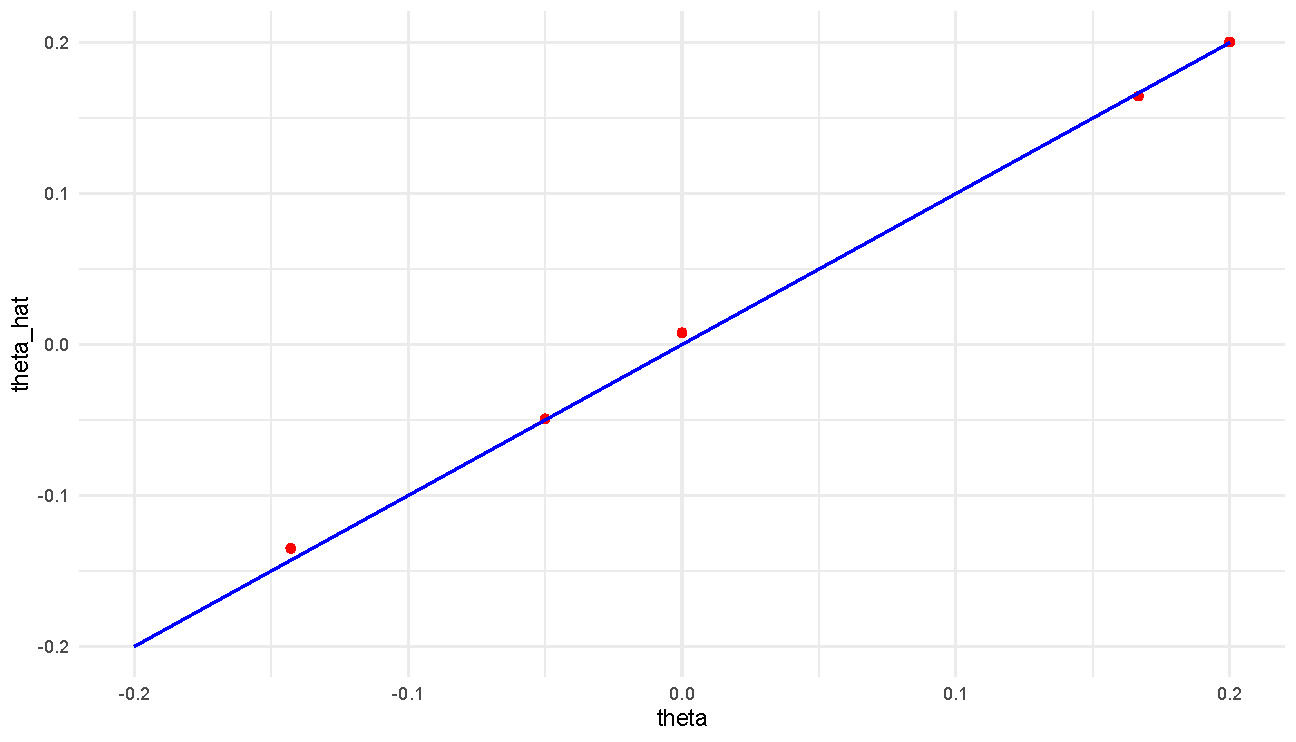
\includegraphics[width=0.8\textwidth]{Mau SP NCKH/image/Approx_theta_with_thetahat2000.pdf}
    \caption{Tham số chuyển $\theta$}
    \label{fig:image2}
  \end{subfigure}

      % Second row with one image centered
  \vspace{0.1cm} % Add vertical space between the rows
  \begin{subfigure}[b]{\textwidth}
    \centering
    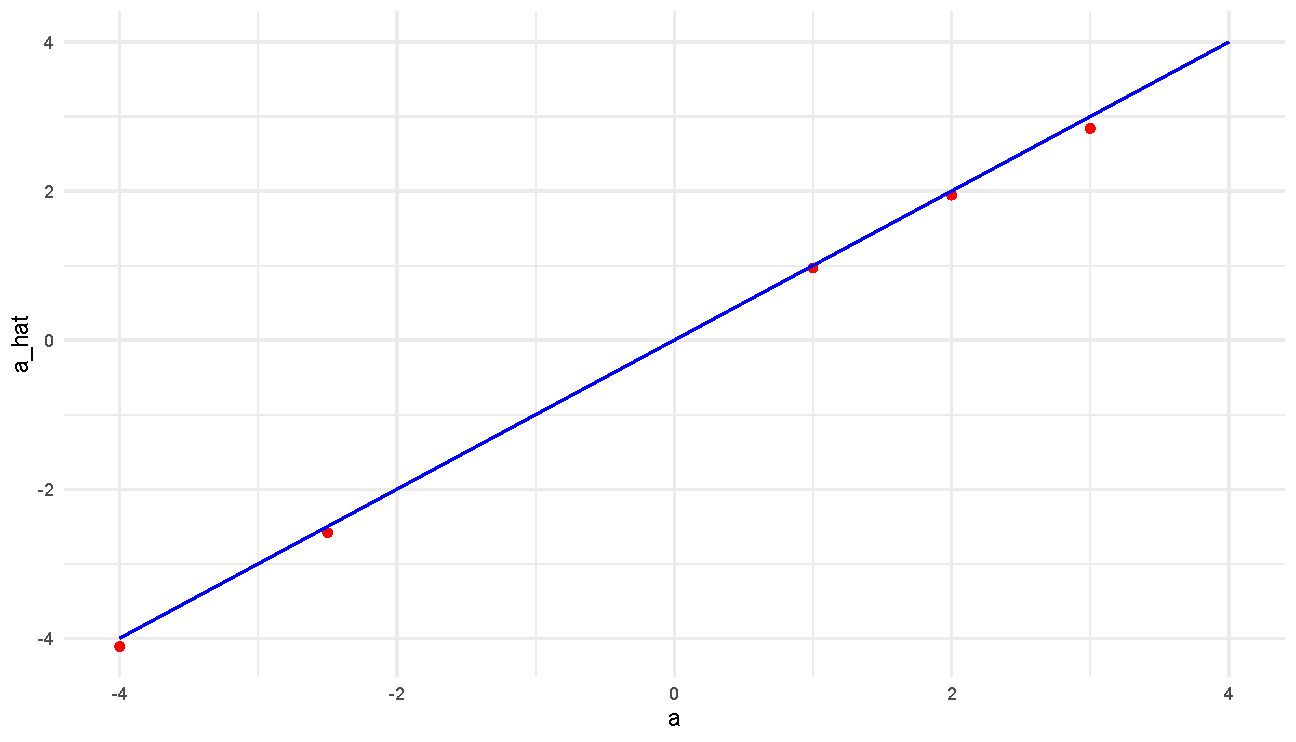
\includegraphics[width=0.4\textwidth]{Mau SP NCKH/image/Approx_a_with_ahat2000.pdf}
    \caption{Tham số co giãn $a$}
    \label{fig:image1}
  \end{subfigure}
  
  \caption{Ước lượng các tham số $v, \theta$ và $a$}
  \label{fig:images-side-by-side}
\end{figure}

\newpage
Hơn nữa, sử dụng sự hội tụ \tref{3.4}, \tref{4.9} và \tref{5.9}, ta có thể nhận được khoảng tin cậy cho các tham số $v, \theta$ và $a$. 
Chẳng hạn, cho $n=2000$, nếu ta đặt $I_{n}\left(v_{2}\right), I_{n}\left(\theta_{3}\right)$ và $I_{n}\left(a_{4}\right)$ là các khoảng tin cậy của $v_{2}, \theta_{1}$ và $a_{1}$, với rủi ro (mức ý nghĩa) $5 \%$, ta có được
$$
\begin{aligned}
I_{n}\left(v_{2}\right) & =[0.243044 ; 0.2920085], \\
\end{aligned}
$$
$$
\begin{aligned}
I_{n}\left(\theta_{1}\right) & =[0.008646117 ; 0.0228825], \\
\end{aligned}
$$
$$
\begin{aligned}
I_{n}\left(a_{1}\right) & =[0.8567415 ;1.005915].
\end{aligned}
$$

Độ dài của các khoảng này lần lượt là $0.0489645,0.01423639$ và 0.1491732. Kết quả là, độ dài của $I_{n}\left(v_{2}\right), I_{n}\left(\theta_{3}\right)$ và $I_{n}\left(a_{4}\right)$ thì nhỏ, nên xác thực khả năng hoạt động hiệu quả của quy trình ước lượng tham số. Tất cả các khoảng tin cậy này được vẽ trong \ref{convergence}.
% \includegraphics[max width=\textwidth, center]{2023_11_01_10532057ac1e795c558bg-15}
\begin{figure}[ht]
  \centering
  \begin{subfigure}[b]{0.45\textwidth}
    \centering
    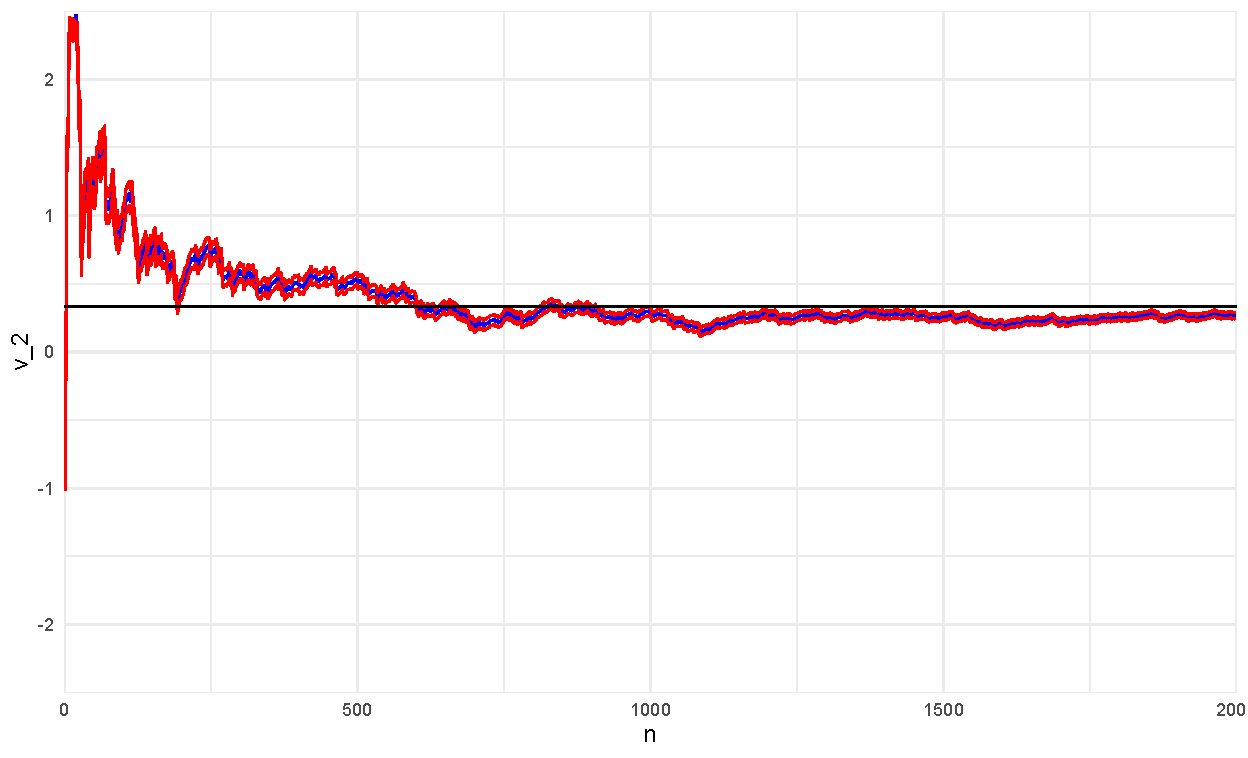
\includegraphics[width=0.8\textwidth]{Mau SP NCKH/image/Convergence/convergence_v_2with_n2000.pdf}
    \caption{Khoảng tin cậy của $v_2$}
    \label{convergence_and_confidence_of_v_1}
  \end{subfigure}
  \hfill % optional; add some horizontal spacing
  \begin{subfigure}[b]{0.45\textwidth}
    \centering
    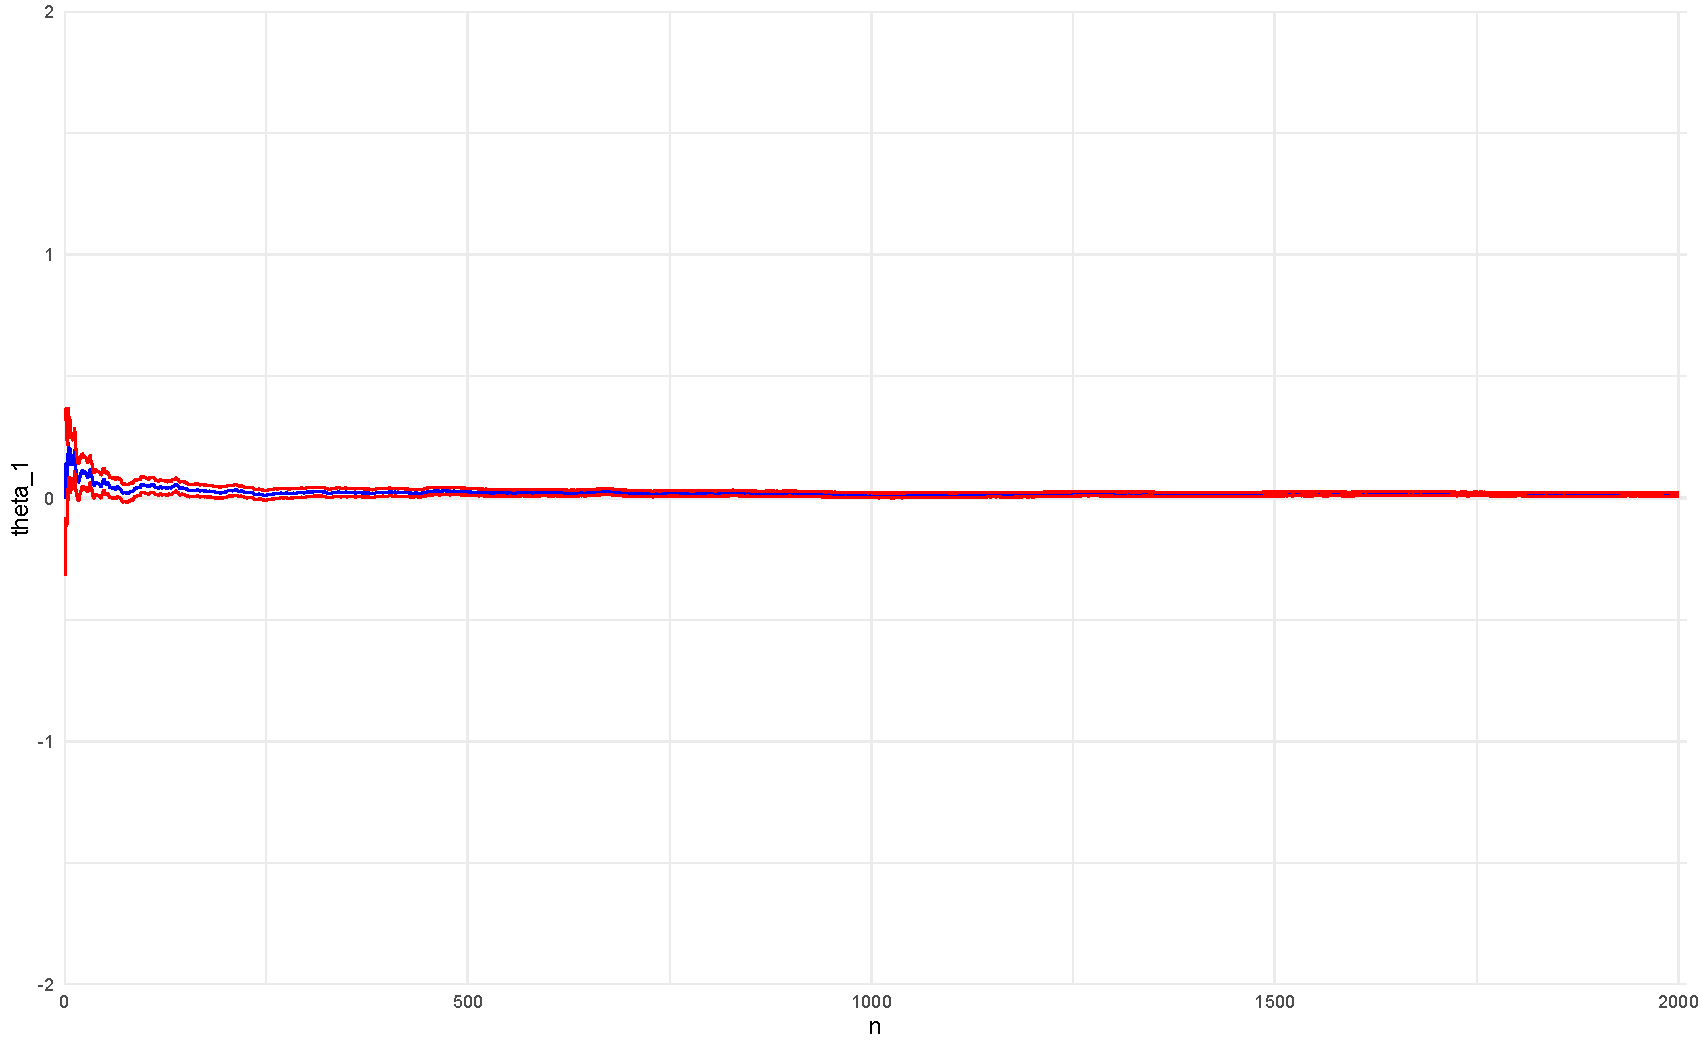
\includegraphics[width=0.8\textwidth]{Mau SP NCKH/image/Convergence/convergence_theta_1with_n2000.pdf}
    \caption{Khoảng tin cậy của $\theta_1$}
    \label{convergence_and_confidence_of_theta_1}
  \end{subfigure}

      % Second row with one image centered
  \vspace{0.1cm} % Add vertical space between the rows
  \begin{subfigure}[b]{\textwidth}
    \centering
    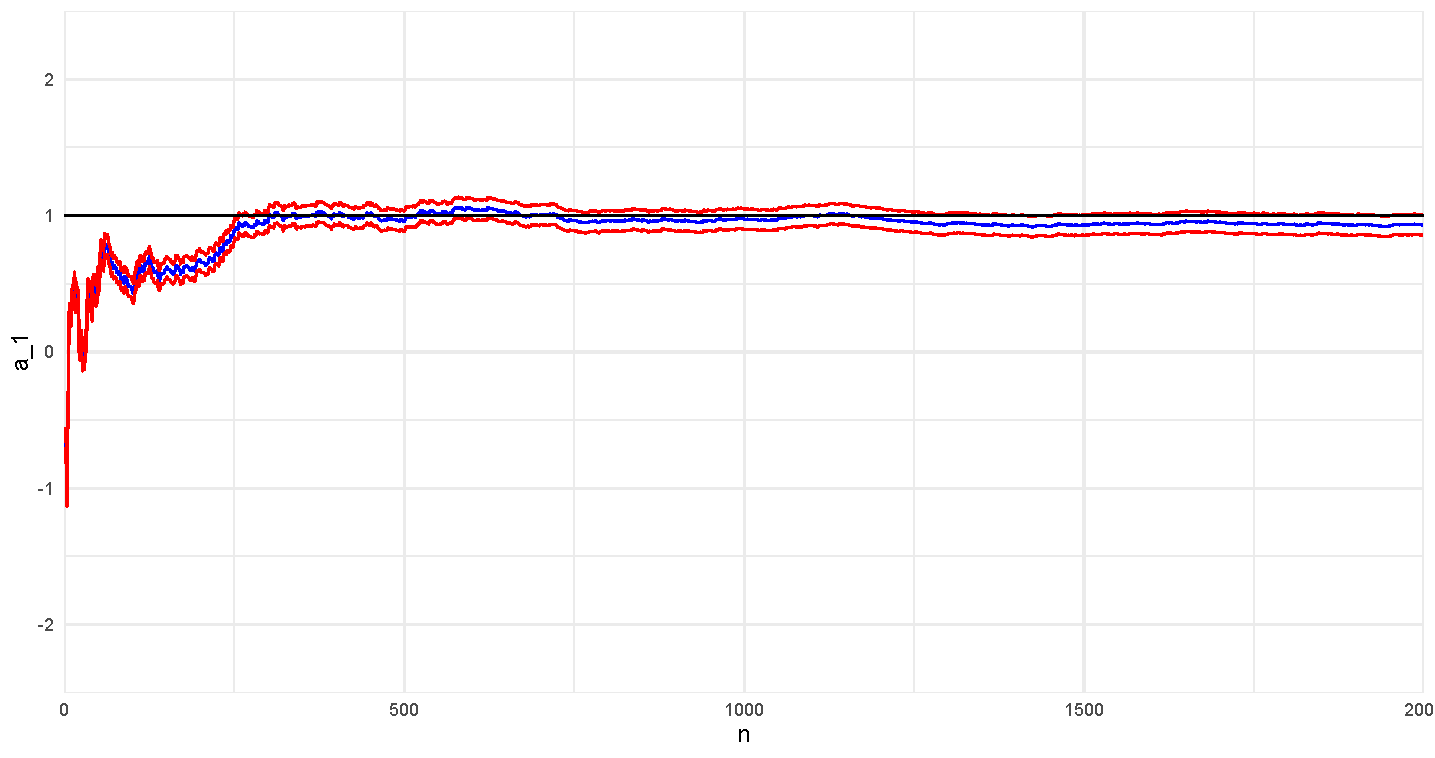
\includegraphics[width=0.4\textwidth]{Mau SP NCKH/image/Convergence/convergence_a_1with_n2000.pdf}
    \caption{Khoảng tin cậy của $a_1$}
    \label{convergence_and_confidence_ofa_1}
  \end{subfigure}
  
  \caption{Khoảng tin cậy của $v_2, \theta_1$ và $a_1$}
  \label{convergence}
\end{figure}


Đối với việc ước lượng hàm hồi quy $f$, ta chọn $\alpha=9 / 10$ cho dãy băng tần $\left(h_{n}\right)$, hàm hạt nhân $K$ sử dụng là hàm hạt nhân đều trên $[-1 ; 1]$ và với mọi $1 \leq j \leq p, \omega_{j}(x)=1 / p$. Việc ước lượng hàm hồi quy $f$ bởi $\widehat{f}_{n}$ được minh họa ở hình bên trái trong hình \ref{convergence_f} , và ước lượng của hàm $f$ bởi $\widehat{f}_{n, 1}$ được minh họa trong hình bên dưới.
\begin{figure}[ht]
  \centering
  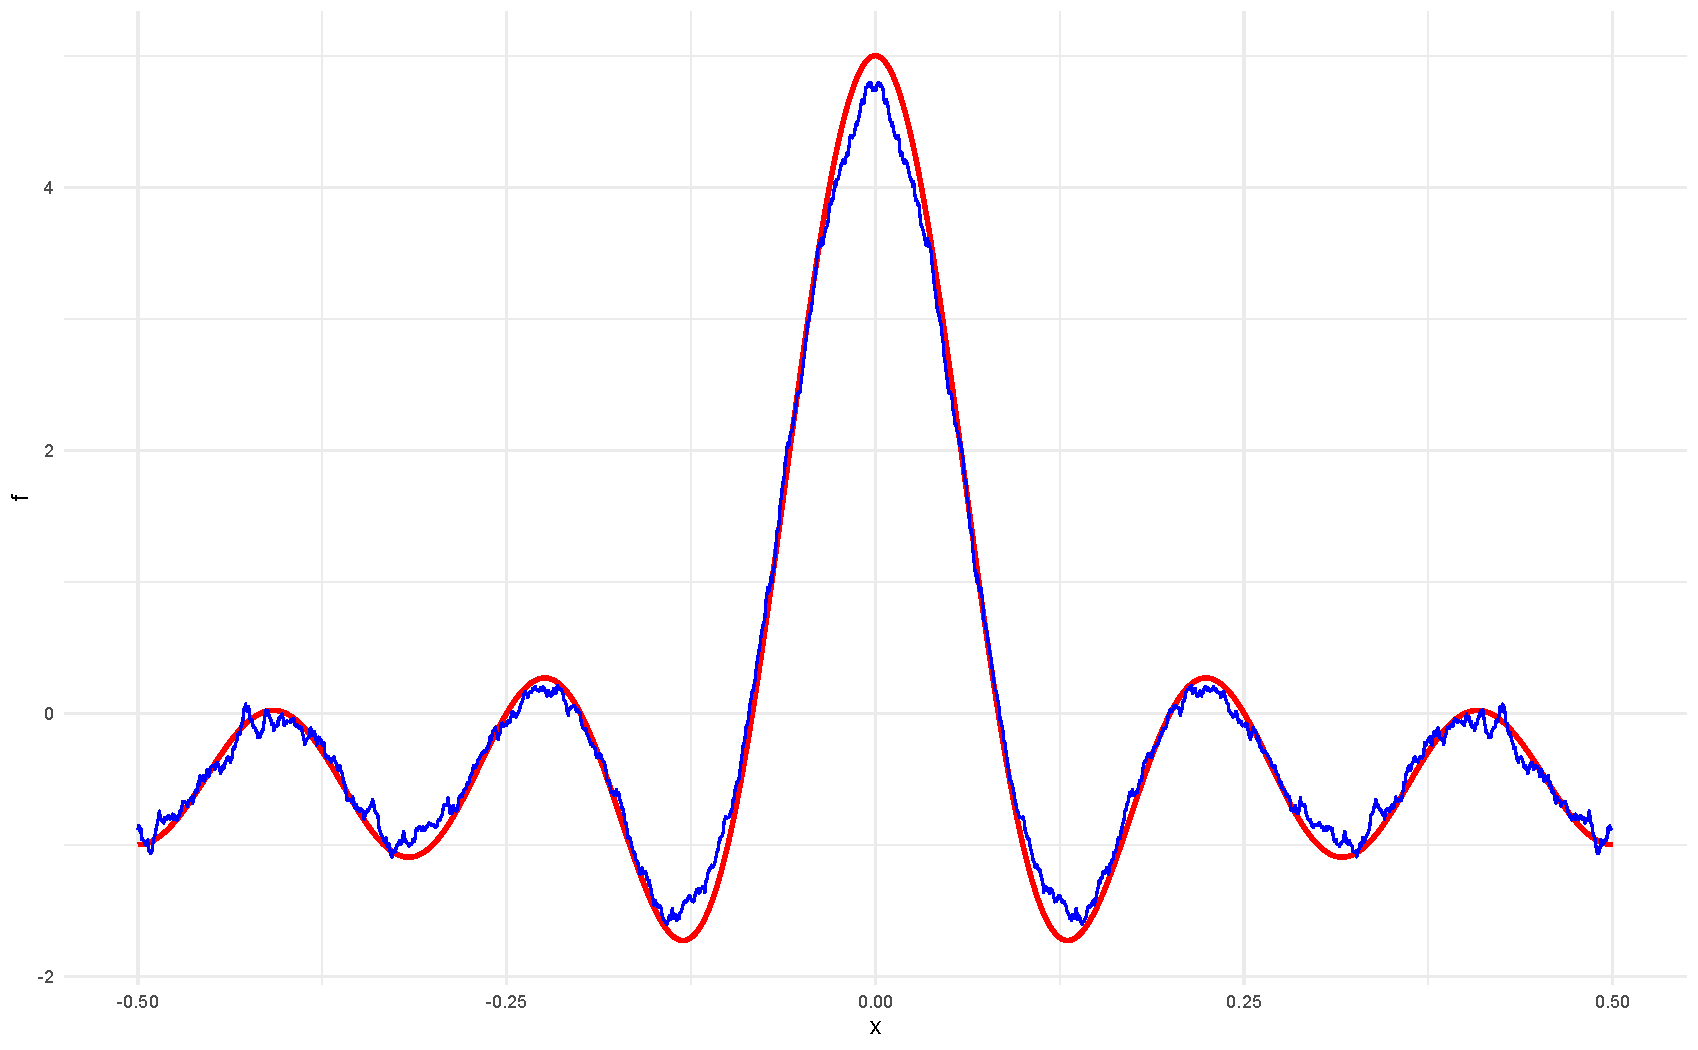
\includegraphics[width=0.65\textwidth]{Mau SP NCKH/image/convergence_f.pdf}
  \caption{Ước lượng hàm $f$ bởi $\hat{f}_n$}
  \label{convergence_f}
\end{figure}
\section{Chương trình R}
Chương trình R để ước lượng các vector tham số $v, \theta, a$  và hàm hồi quy $f$ chia làm sáu phần. Đầu tiên là phần định nghĩa các hàm được sử dụng trong chương trình, sau đó ta sẽ khởi tạo dữ liệu mô phỏng được định nghĩa ở mục trước, tiếp đến lần lượt là các phần chương trình để ước lượng các vector tham số $v, \theta, a$ và phần chương trình cuối cùng - phần thứ sáu sẽ ước lượng hàm hồi quy $f$
\begin{lstlisting}[language=R, title = Phần 1: Các hàm sử dụng trong chương trình]
##########
### Chuan bi cac ham su dung trong chuong trinh
library(ggplot2)
library(ICSNP)
set.seed(45)  # Thiet lap seed de tai tao ket qua
T.test <- function(X, mu=0){
  X <- as.matrix(X)
  n <- nrow(X)
  p <- ncol(X)
  df2 <- n - p
  if(df2 < 1L) stop("Need nrow(X) > ncol(X).")
  if(length(mu) != p) mu <- rep(mu[1], p)
  xbar <- colMeans(X)
  S <- cov(X)
  T2 <- n * t(xbar - mu) %*% solve(S) %*% (xbar - mu)
  Fstat <- T2 / (p * (n-1) / df2)
  pval <- 1 - pf(Fstat, df1=p, df2=df2)
  data.frame(T2=as.numeric(T2), Fstat=as.numeric(Fstat),
             df1=p, df2=df2, p.value=as.numeric(pval), row.names="")
}


T.ci <- function(mu, Sigma, n, avec=rep(1,length(mu)), level=0.95){
  p <- length(mu)
  if(nrow(Sigma)!=p) stop("Need length(mu) == nrow(Sigma).")
  if(ncol(Sigma)!=p) stop("Need length(mu) == ncol(Sigma).")
  if(length(avec)!=p) stop("Need length(mu) == length(avec).")
  if(level <=0 | level >= 1) stop("Need 0 < level < 1.")
  cval <- qf(level, p, n-p) * p * (n-1) / (n-p)
  zhat <- crossprod(avec, mu)
  zvar <- crossprod(avec, Sigma %*% avec) / n
  const <- sqrt(cval * zvar)
  c(lower = zhat - const, upper = zhat + const)
}


rma <- function(x, p, r = TRUE){
  # Mo rong ma tran theo hang va cot
  # matrix                  x: ma tran dau vao
  # line of extend          p: So dong muon mo rong
  # direction of extension  r: TRUE neu mo rong theo hang, FALSE neu mo rong theo cot
  # state: da kiem tra ham nay la dung
  c_or_r = x
  if(r == TRUE){
    for(i in 2:p){
      x = rbind(x,c_or_r)
    }
  }else{
    for(i in 2:p){
      x = cbind(x,c_or_r)
    }
  }
  return(x)
}


sum_broadcast <- function(a,b){
  # a va b lan luot tuong ung voi ma tran co so chieu dim (p,1) and (1,p)
  return(rma(a,dim(b)[2],r=FALSE)+rma(b,dim(a)[1]))
}


D <- function(X,t,p=5){
  # state: da kiem tra ham nay la dung
  # input X: mot bien ngau nhien, EX: X[1,1]
  g = 1
  t = matrix(t,nrow=length(t), ncol=1)
  s = (1/g)*c(sin(2*pi*(X-t[1,])))
  for(i in 2:p){
    s = c(s,(1/g)*sin(2*pi*(X-t[i,])))
  }
  return(diag(s))
}


my_f <- function(x) {    
  out <- cos(2*pi*(x))*(cos(2*pi*1*(x)) + cos(2*pi*2*(x)) + cos(2*pi*3*(x)) + cos(2*pi*4*(x)) + cos(2*pi*5*(x)))
  return(out)
}


f1 <- integrate(my_f,          # Ap dung tinh tich phan trong R
                lower = -1/2,
                upper = 1/2)


f <- function(x){
  out2 <- cos(2*pi*1*(x))+cos(2*pi*2*(x))+cos(2*pi*3*(x))+cos(2*pi*4*(x))+cos(2*pi*5*(x))
  return(out2)
}

Vectorize_f <- Vectorize(f)
\end{lstlisting}

\begin{lstlisting}[language=R, title = Phần 2: Tạo dữ liệu mô phỏng]
p =  5
n = 2000
g = 1
rowx <- runif(n, min=-0.5,max= 0.5)  # Tao gia tri x
x = matrix(rowx,nrow = 1,ncol = length(rowx))
x = rma(x,p=p)

# Chuan bi cac vecto v, theta, a and esp
v = matrix(c(0,1/3,-1,2,-9/10),nrow=p,ncol=1)
theta = matrix(c(0,1/5,-1/20,-1/7,1/6),nrow=p,ncol=1)
a = matrix(c(1,-4,3,-5/2,2),nrow=p,ncol=1)


##
f_vec <- Vectorize(f)
gamma_j <-  1/(2*pi*a*(1/2))
##

esp = matrix(rnorm(n*p, mean = 0, sd = 1), nrow=p)
Y = (rma(a, n, r= FALSE))*f_vec(x-rma(theta,n,r=FALSE)) + rma(v,n, r=FALSE) + esp

# Khi ma bind xong thi Y la matrix

# dataframe
df <- data.frame(
  x = c(t(x)),
  y = c(t(Y)),
  wave = factor(c(rep('a_1,theta_1,v_1', n),
                  rep('a_2,theta_2,v_2', n),
                  rep('a_3,theta_3,v_3', n),
                  rep('a_4,theta_4,v_4', n),
                  rep('a_5,theta_5,v_5', n))))

# Tao cac bieu do duong
ggplot(df, aes(x = x, y = y, color = wave)) + 
  geom_line() +  # Them cac lop chi tiet cho bieu do
  xlab('x') +
  ylab('y') +
  theme_minimal() +
  scale_color_manual(values = c('blue', 'red', 'green', 'purple', 'yellow'))
\end{lstlisting}
Ước lượng tham số chiều cao $v$
\begin{lstlisting}[language=R, title = Phần 3: Ước lượng tham số chiều cao]
##################################################
# Uoc luong tham so chuyen v
# Tinh v_n
v_n = matrix(diag(diag(p))-0.75, nrow=p, ncol=1)
cv = 0
for(i in 2:n){
  cv <- 0
  for(j in 1:i){
    cv <- cv + (1/i)*Y[,j]/g  # This calculates average per row
  }
  v_n <- cbind(v_n, (cv))  
}
\end{lstlisting}
\begin{lstlisting}[language=R,title = Phần 4: Ước lượng tham số chuyển]
##################################
# Estimate theta parameters
f1_hat <- function(x,Y,n, g = 1){
  # x is vector EX: x[1,]
  # y is vector EX: Y[1,]
  x = matrix(x,nrow = 1)
  Y = matrix(Y,ncol = 1)
  return((1/n)*((cos(2*pi*x)/g)%*%Y))
}

# f1_hat = (1/n)*matrix(cos(2*pi*x[1,]),nrow = 1)%*%matrix(Y[1,],nrow = length(Y[1,]))  

C <- function(X,t,p=5){
  g = 1
  t = matrix(t,nrow=length(t), ncol=1)
  s = (1/g)*c(cos(2*pi*(X-t[1,])))
  for(i in 2:p){
    s = c(s,(1/g)*cos(2*pi*(X-t[i,])))
  }
  return(diag(s))
}
# Estimate theta
pi_K <- function(x) {
  #state: checked
  ifelse(abs(x) <= 1/4, x, ifelse(x > 1/4, 1/4, -1/4))
}
pi_K_vectorized <- Vectorize(pi_K) # Tra ve mot day so co tri tuyet doi nho hon hoac bang 0.25

N = n
gamma <- 1/ (1:n)  
theta_hat = c(0,0,0,0,0)
matrix_theta =  matrix(theta_hat, ncol=1)

# Uoc luong theta
for (nn in 1:(N-1)) { #(N-1)
  T_np <- D(x[1,nn+1],theta_hat)%*%matrix(Y[,nn+1],nrow=p,ncol=1) # Assuming Y_n = 1 and g(X_n) = 1 (uniform density)
  index = nn + 1
  theta_hat <- pi_K_vectorized(matrix(theta_hat,nrow=p,ncol=1) + (gamma_j*gamma[index]) * T_np)
  matrix_theta = cbind(matrix_theta, theta_hat)
}
\end{lstlisting}
\newpage
\begin{lstlisting}[language=R, title = Phần 5: Ước lượng tham số co giãn]
###############################################################################
# Uoc luong asim
C <- function(X,t,p=5){
  g = 1
  t = matrix(t,nrow=length(t), ncol=1)
  s = (1/g)*c(cos(2*pi*(X[1,]-t[1,])))
  if(p >= 2){
    for(i in 2:p){
      s = c(s,(1/g)*cos(2*pi*(X[i,]-t[i,])))
    }  
  }
  return(diag(s))
}

vector_asim = (1/(2*f1$value))*diag(C(matrix(x[1,2:2],ncol=1), matrix_theta[1,1:(2-1)],p=2-1))%*%matrix(Y[1,2:2],ncol = 1)
matrix_asim = matrix(0, nrow = 1, ncol = n - 2)
for(j in 1:p){
  for(i in 3:n){
    asim_i = (1/(i*f1$value)*diag(C(matrix(x[1,2:i],ncol=1), matrix_theta[j,1:(i-1)],p=i-1))%*%matrix(Y[j,2:i],ncol = 1))
    vector_asim = c(vector_asim, asim_i)
  }
  matrix_asim <- rbind(matrix_asim, matrix(vector_asim,nrow = 1))
  vector_asim = (1/(2*f1$value))*diag(C(matrix(x[1,2:2],ncol=1), matrix_theta[j,1:(2-1)],p=2-1))%*%matrix(Y[j,2:2],ncol = 1)
}
matrix_asim = matrix_asim[2:dim(matrix_asim)[1], ]
last_col <- matrix(matrix_asim[,n-(n - dim(matrix_asim)[2] + 1)], ncol = 1)
for(i in 1:(n - dim(matrix_asim)[2])){
  matrix_asim <- cbind(matrix_asim, last_col)
}
\end{lstlisting}
\begin{lstlisting}[language=R, title = Phần 6: Ước lượng hàm hồi quy $f$ và vẽ hình minh họa]
###########################################################################
# Da chuan bi xong v_n, matrix_theta, matrix_asim
# Tien hanh uoc luong ham hoi quy f
fn_hat <- function(x, kernel, n = 1500){
  weight = diag(1/p*diag(1,p,p))
  alpha = 9/10
  x = matrix(x,nrow = 1, ncol = n)
  
  
  
  # uniform_kernel_vectorized return sequence c()
  h = matrix(c(1:n), nrow = 1)**alpha
  xn = matrix(x[,1:n], nrow = 1)
  for(j in 1:p){
    thetan_j = matrix(matrix_theta[j,1:n], nrow = 1)
    xn = xn - thetan_j - x
    inpK = (1/h)*xn
  }  
}

uniform_kernel <- function(u) {
  # Ap dung ham hat nhan deu
  # K(u) = 1/2 if |u| <= 1, neu khong thi K(u) = 0
  ifelse(abs(u) <= 2, 1/4, 0)
}

uniform_kernel_vectorized <- Vectorize(uniform_kernel)

gaussian_kernel <- function(u) {
  # Ham hat nhan Gauss
  1 / sqrt(2 * pi) * exp(-u^2 / 2)
}

gaussian_kernel_vectorized <- Vectorize(gaussian_kernel)

inpK <- function(xn, theta, x, h){
  # Kiem soat input dau vao
  xn = matrix(xn, nrow = 1)
  theta = matrix(theta, nrow = 1)
  x = matrix(x, nrow = 1)
  h = matrix(h, nrow = 1)
  
  xn = xn - theta - x
  inpK = (1/h)*xn
  return(inpK)
}
# uniform_kernel_vectorized tra ve mot day seq()
weight = matrix(diag(1/p*diag(1,p,p)), nrow = 1)
alpha = 9/10
matrix_fn_hat = seq()
nopoint = 2000
for(i in 3:nopoint){
  h = (1/matrix(c(1:n), nrow = 1, ncol = n))**alpha
  xn = matrix(x[1,1:n], nrow = 1)
  x1 = matrix(seq(-0.5,0.5, length.out = nopoint)[i],nrow = 1, ncol = n) 
  matrix_fn_hat_j = seq()
  for(j in 1:p){
    thetan_j = matrix(c(matrix_theta[j,1],matrix_theta[j,1:n-1]), nrow = 1, ncol = n)
    inpKp = inpK(xn, thetan_j,  x1, h)
    inpKm = inpK(xn, thetan_j, -x1, h)
    matrixKp = matrix(uniform_kernel_vectorized(inpKp),nrow = 1)
    matrixKm = matrix(uniform_kernel_vectorized(inpKm),nrow = 1)
    Swp = (1/h)*matrixKp
    Swm = (1/h)*matrixKm
    Sw = (Swp + Swm)
    
    fsim_j = matrix(Y[j,1:n],ncol = 1) - matrix(c(v_n[j,1],v_n[j,1:n-1]), ncol = 1)
    
    fn_hat_j = (1/matrix_asim[j,n])*(Sw%*%fsim_j)/sum(Sw)
    matrix_fn_hat_j = c(matrix_fn_hat_j, fn_hat_j[1])
  }
  fn_hat = weight%*%matrix(matrix_fn_hat_j[2:length(matrix_fn_hat_j)], ncol = 1, nrow = length(matrix_fn_hat_j[2:length(matrix_fn_hat_j)]))
  matrix_fn_hat = c(matrix_fn_hat, fn_hat)
}
  
#############################################################################
# dataframe
df <- data.frame(
  x = c(seq(-0.5,0.5, length.out=nopoint-1)),
  y = c(matrix(matrix_fn_hat[2:n],ncol = 1, nrow = n-1)))
  y_true = Vectorize_f(c(seq(-0.5,0.5, length.out=nopoint-1)))


# Ve bieu do hoi tu cua uoc luong f_hat_n ve ham f
ggplot() +  
  geom_line(data = df, aes(x = x, y = y_true), color = 'red', size = 1)+
  geom_line(data = df, aes(x = x, y = y), color = 'blue')+   # Them cac chi tiet cho bieu do
  xlab('x') +
  ylab('f') +
  theme_minimal() +
  scale_color_manual(values = c('blue', 'red', 'green', 'purple', 'green'))



\end{lstlisting}
%Hơn nữa, theo sự hội tụ \tref{6.6} và \tref{6.7}, cho $n=2000$ và với mọi $x \in[-1 / 2 ; 1 / 2]$, 

%Ta có sự hội tụ của hàm $\widehat{f}_n$ về $f$ như trong hình 4.4
% khoảng tin cậy của $f(x)$ xác định bởi
% $$
% K_{n}(x)=\left[\widehat{f}_{n}(x)-q_{\beta} \frac{\widehat{w}_{n}\left(x, \widehat{\theta}_{n}\right)}{\sqrt{n h_{n}}}, \widehat{f}_{n}(x)+q_{\beta} \frac{\widehat{w}_{n}\left(x, \widehat{\theta}_{n}\right)}{\sqrt{n h_{n}}}\right]
% $$
% trong đó ta có thể suy ra từ sự hội tụ \tref{3.3} và \tref{3.4} của Định lý 3.2 trong \cite{bercu} rằng cho $n=2000$ và với mọi $x \in[-1 / 2 ; 1 / 2]$, một khoảng tin cậy cho hàm $f(x)$ xác định bởi
% $$
% J_{n}(x)=\left[\widehat{f}_{n, 1}(x)-q_{\beta} \frac{\widehat{v}_{n}\left(x, \widehat{\theta}_{n, 1}\right)}{\sqrt{n h_{n}}}, \widehat{f}_{n, 1}(x)+q_{\beta} \frac{\widehat{v}_{n}\left(x, \widehat{\theta}_{n, 1}\right)}{\sqrt{n h_{n}}}\right]
% $$
% trong đó $q_{\beta}$ phân vị cấp $0<\beta<1$ của phân phối $\mathcal{N}(0,1)$ và $\widehat{w}_{n}^{2}\left(x, \widehat{\theta}_{n}\right)$ và $\widehat{v}_{n}^{2}\left(x, \widehat{\theta}_{n, 1}\right)$ là một ước lượng vững của phương sai tiệm cận của $w^{2}(x, \theta)$ trong Định lý 6.2 và của $v^{2}\left(x, \theta_{1}\right)$ trong Định lý 3.2 của \cite{bercu}. Trong trường hợp này $\nu^{2}=1 / 2$, và một tính toán số học dẫn đến
% $$
% w^{2}(x, \theta)= \begin{cases}0.0114 & \text { nếu }-1 / 2 \leq x \leq-23 / 50 \text { và } 23 / 50 \leq x \leq 1 / 2, \\ 0.0108 & \text { nếu }-23 / 50<x \leq-9 / 25 \text { và } 9 / 25 \leq x<23 / 50 \\ 0.0099 & \text { nếu }-9 / 25<x \leq-17 / 50 \text { và } 17 / 50 \leq x<9 / 25 \\ 0.0086 & \text { nếu }-17 / 50<x \leq-31 / 100 \text { và } 31 / 100 \leq x<17 / 50, \\ 0.0083 & \text { nếu }-31 / 100<x<0 \text { và } 0<x<31 / 100, \\ 0.0166 & \text { nếu } x=0,\end{cases}
% $$
% và
% $$
% v^{2}\left(x, \theta_{1}\right)= \begin{cases}5 / 38 & \text { nếu } x \neq 0 \\ 5 / 19 & \text { nếu } x=0\end{cases}
% $$
% Nói cách khác, với mọi $x \in[-1 / 2 ; 1 / 2]$, bậc của phương sai tiệm cận $v^{2}\left(x, \theta_{1}\right)$ nhận được từ ước lượng $\widehat{f}_{n, 1}$ gấp hơn mười lần so với bậc của phương sai tiệm cận $w^{2}(x, \theta)$ nhận được từ $\widehat{f}_{n}$. Thêm vào đó, trong trường hợp này, phương sai tối đa được cho trong Chú ý 6.2 là, với mọi $x \in[-1 / 2 ; 1 / 2]$, có bậc $10^{-3}$ nhỏ hơn $w^{2}(x, \theta)$ mười lần. Các khoảng tin cậy $K_{n}(x)$ và $J_{n}(x)$ được vẽ bằng màu đỏ trong Figure 5. Ta có thể thấy trong Figure 4 rằng ước lượng $\widehat{f}_{n}$ thì gần hàm $f$ hơn $\widehat{f}_{n, 1}$. Chính xác hơn, ước lượng của hàm $f$ bởi $\widehat{f}_{n}$ thì tốt hơn ước lượng bởi $\widehat{f}_{n, 1}$ vì độ dài khoảng tin cậy $K_{n}(x)$ thì nhỏ hơn độ dài $J_{n}(x)$ như có thể thấy được trong Figure 5, tùy thuộc vào bậc của hai phương sai $v^{2}\left(x, \theta_{1}\right)$ và $w^{2}(x, \theta)$. Trong trường hợp của ta,  khoảng tin cậy lớn nhất $K_{n}(x)$ có độ dài 0.3460 (khi $x=0$ ) và nhỏ hơn gần ba lần so với $J_{n}(x) = 0.9723$ (khi $x=-0.09$ và $x=0.09)$. Cụ thể hơn, điều này khẳng định lựa chọn phiên bản ước lượng Nadaraya-Watson có trọng.
% %\includegraphics[max width=\textwidth, center]{2023_11_01_10532057ac1e795c558bg-17(1)}

% Figure 4 . Ước lượng hàm $f$ bởi $\widehat{f}_{n}$ và $\widehat{f}_{n, 1}$
% %\includegraphics[max width=\textwidth, center]{2023_11_01_10532057ac1e795c558bg-17}

% Figure 5. Các khoảng tin cậy của hàm $f$



% \subsection{Nội dung xây dựng thuật toán}
% Tôi xem xét
% \verb|x| là một ma trận p dòng và n cột, $\mathbf{x} \in \mathbb{R}^{p\times n}$
% \verb|x| là một ma trận p dòng và n cột, $\mathbf{x} \in \mathbb{R}^{p\times n}$
